\chapter{Business Intelligence Workload}
\label{sec:bi}

The LDBC SNB BI workload consists of two sets of operations:

\begin{itemize}
\item \textbf{Read queries.} Complex read queries touching a significant portion of the data. See \autoref{sec:bi-reads}.
\item \textbf{Microbatches of update operations.} A set of insert and delete operations, batched for a given time period (\eg an hour, a day, \etc). See Sections \ref{sec:bi-insert-operations} and \ref{sec:bi-delete-operations}.
\end{itemize}

\section{Benchmark Scenario}
\label{sec:bi-benchmark-scenario}

\begin{figure}[H]
    \centering
    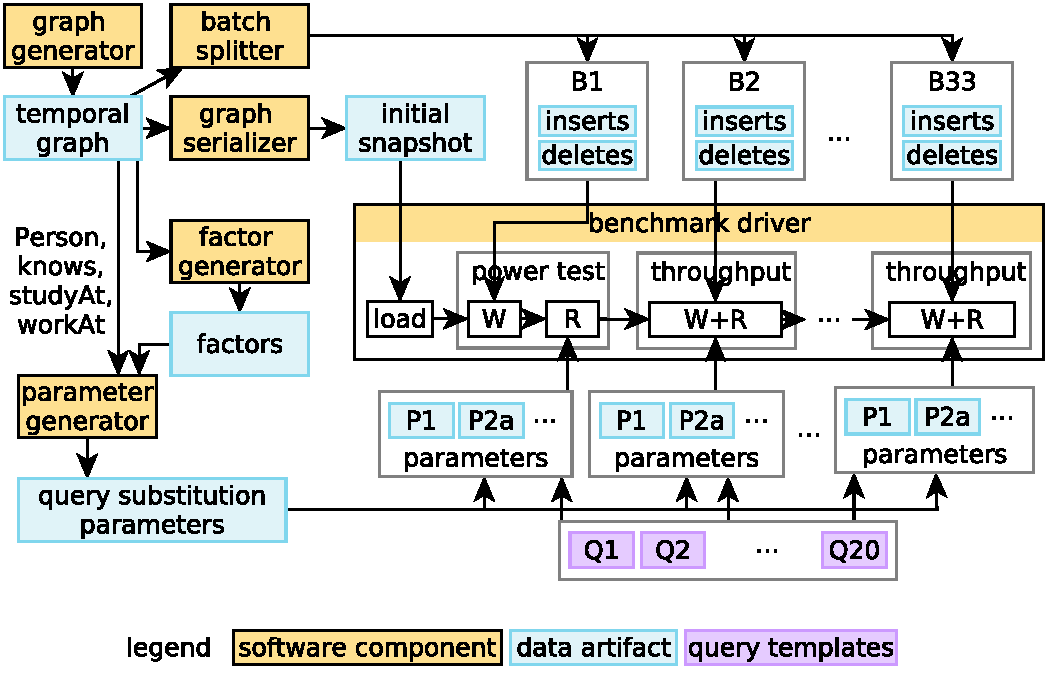
\includegraphics[scale=\yedscale]{figures/bi-workflow}
    \caption{Main software components and data artifacts of the benchmark and their connection to the workflow executed by the BI benchmark driver. Note that unlike SNB Interactive, the BI workload does not have a warmup period.}
    \label{fig:bi-workflow}
\end{figure}

The workflow of the BI workload is shown in \autoref{fig:bi-workflow}.
The read query variants (Q1, Q2a, \ldots) are executed with 30~different substitution parameters in each batch.

\section{Parameter Selection}
\label{sec:bi-paramgen}

During data generation, a sequence of \emph{substitution parameters}
\iftoggle{StandaloneWorkloadSpecification}{}{(\autoref{sec:substitution-parameters})}
is generated.
Similarly to the Interactive workload, the parameter generation of the BI workload uses \emph{parameter curation}~\cite{DBLP:conf/tpctc/GubichevB14} to ensure that the query runtimes are  predictable (to some extent).

Several queries use multiple variants with different sets of input parameters.
\Eg for \queryRefCard{bi-read-14}{BI}{14}, 14(A) uses close countries while 14(B) uses countries that are far from each other.

In principle, query parameters are selected so that the query touches on a similar amounts of data.
For queries which are only constrained by one parameter, we select ranges in the distribution where the starting node has a similar amount of neighbours.
For example, if the query looks for \tMessages with a given \tTag:
(1) the Datagen computes the frequency of \tMessages per \tTags as a factor table,
(2) for each \tTag, we compute its distance (absolute difference) from a given percentile of the distribution is selected (\eg the \tTag on the 75th percentile),
(3) we pick the $k$ parameters with the lowest distance.

\subsection*{Related Publications}

The draft BI workload was published at the \mbox{GRADES-NDA} workshop at \mbox{SIGMOD 2018}~\cite{DBLP:conf/grades/SzarnyasPAMPKEB18}.

%%%%%%%%%%%%%%%%%%%%%%%%%%%%%%%%%%%%%%%%%%%%%%%%%%%%%%%%%%%%%%%%%%%%%%%%%%%%%%
%%%%%%%%%%%%%%%%%%%%%%%%%%%%%%%%%%%%%%%%%%%%%%%%%%%%%%%%%%%%%%%%%%%%%%%%%%%%%%
%%%%%%%%%%%%%%%%%%%%%%%%%%%%%%%%%%%%%%%%%%%%%%%%%%%%%%%%%%%%%%%%%%%%%%%%%%%%%%

\section{Reads}
\label{sec:bi-reads}

\input{query-cards/bi-read-01}
\input{query-cards/bi-read-03}
\input{query-cards/bi-read-04}
\input{query-cards/bi-read-05}
\input{query-cards/bi-read-06}
\input{query-cards/bi-read-07}
\input{query-cards/bi-read-08}
\input{query-cards/bi-read-10}
\input{query-cards/bi-read-14}
\input{query-cards/bi-read-16}
\input{query-cards/bi-read-17}
\input{query-cards/bi-read-18}
\input{query-cards/bi-read-21}
\input{query-cards/bi-read-22}
\input{query-cards/bi-read-25}

% reset counter to make sure the last query card isn't stuck in highlighted mode
\renewcommand{\currentQueryCard}{0}


%%%%%%%%%%%%%%%%%%%%%%%%%%%%%%%%%%%%%%%%%%%%%%%%%%%%%%%%%%%%%%%%%%%%%%%%%%%%%%
%%%%%%%%%%%%%%%%%%%%%%%%%%%%%%%%%%%%%%%%%%%%%%%%%%%%%%%%%%%%%%%%%%%%%%%%%%%%%%
%%%%%%%%%%%%%%%%%%%%%%%%%%%%%%%%%%%%%%%%%%%%%%%%%%%%%%%%%%%%%%%%%%%%%%%%%%%%%%

\section{Insert Operations}
\label{sec:bi-insert-operations}

Insert operations consist of individual inserts for each entity type.
Implementations typically use the same format as the one for loading the initial snapshot of the data set.

%%%%%%%%%%%%%%%%%%%%%%%%%%%%%%%%%%%%%%%%%%%%%%%%%%%%%%%%%%%%%%%%%%%%%%%%%%%%%%
%%%%%%%%%%%%%%%%%%%%%%%%%%%%%%%%%%%%%%%%%%%%%%%%%%%%%%%%%%%%%%%%%%%%%%%%%%%%%%
%%%%%%%%%%%%%%%%%%%%%%%%%%%%%%%%%%%%%%%%%%%%%%%%%%%%%%%%%%%%%%%%%%%%%%%%%%%%%%

\section{Delete Operations}
\label{sec:bi-delete-operations}
\iftoggle{StandaloneWorkloadSpecification}{
    \input{query-cards/delete-01}
\input{query-cards/delete-02}
\input{query-cards/delete-03}
\input{query-cards/delete-04}
\input{query-cards/delete-05}
\input{query-cards/delete-06}
\input{query-cards/delete-07}
\input{query-cards/delete-08}

}{
    See \autoref{sec:delete-operations}.
}
